\documentclass{beamer}
\mode<presentation>
{
	\usetheme{Madrid}      % or try Darmstadt, Madrid, Warsaw, ...
	\usecolortheme{default} % or try albatross, beaver, crane, ...
	\usefonttheme{default}  % or try serif, structurebold, ...
	\setbeamertemplate{navigation symbols}{}
	\setbeamertemplate{caption}[numbered]
} 
\usepackage[english]{babel}
\usepackage[utf8x]{inputenc}

\usepackage{graphicx} % Allows including images
\usepackage{booktabs} % Allows the use of \toprule, \midrule and \bottomrule in tables

\usepackage{tikz}
\usepackage[ruled,linesnumbered]{algorithm2e}
\usetikzlibrary{shapes,snakes}

\usepackage{url}
\usepackage{appendixnumberbeamer}


\newcommand{\norm}[1]{\left\lVert#1\right\rVert}
\newcommand{\argmin}{\arg\!\min}

% more on the introduction
% => possible explanations
% hard to follow the sentenses
% 


\title{Text Classification with Generic Logistic-Regression Classifier}
\author{Marc Moreaux}
\institute{Aalborg university}
% \date{\today}

\begin{document}

	%#########################################
	%##  TITLE 
	\begin{frame}
		\titlepage
	\end{frame}



	%#########################################
	%##  PROBLEM STATEMENT
	\begin{frame}{Project objective}

		\begin{block}{}
			Classify a dataset of unknown nature with logistic-regression using hand-engineered features.
		\end{block}

	\end{frame}


	% %#########################################
	% %##  PROBLEM STATEMENT
	% \begin{frame}{Project objective}

	% 		\begin{figure}
	% 			\centering
	% 			\def\layersep{3em}

	% 			\begin{tikzpicture}[shorten >=1pt,->,draw=black!50, node distance=\layersep]
	% 				\tikzstyle{every pin edge}=[<-, thick,shorten >=1pt]
	% 				\tikzstyle{neuron}=[circle,draw=black, very thick,,minimum size=1.5em,inner sep=0em]
	% 				\tikzstyle{annot} = [text width=9em, text centered]
	% 				\tikzstyle{annot2} = [text width=6em, text centered]

	% 				% --------------
	% 				%   Draw nodes
	% 				% --------------
	% 				\node[neuron] (O) at (3.5,\layersep*3) {}; % Draw output node

	% 				\foreach \name / \y in {1,...,6} % Draw the inputs nodes
	% 					\node[neuron] (H2-\name) at (\y+0.0,\layersep*2) {};

	% 				% -----------------
	% 				%   Connect nodes
	% 				% -----------------
	% 				\foreach \source in {1,...,6} % connect inputs & out
	% 						\path (H2-\source) edge (O);

	% 			\end{tikzpicture}

	% 			\caption{Example of logistic regression model}
	% 			\label{fig:DNN}
	% 		\end{figure}

	% \end{frame}


	%#########################################
	%##  PROBLEM STATEMENT
	\begin{frame}{Paper objective}

		\tableofcontents

	\end{frame}



	%####################################################################################################### 
	%####################################################################################################### Competition description
	%####################################################################################################### 


	%#########################################
	%##  doc example
	\section{Competition description}
	\begin{frame}{Competition description}
	
		\begin{figure}[h]
			\begin{center}
				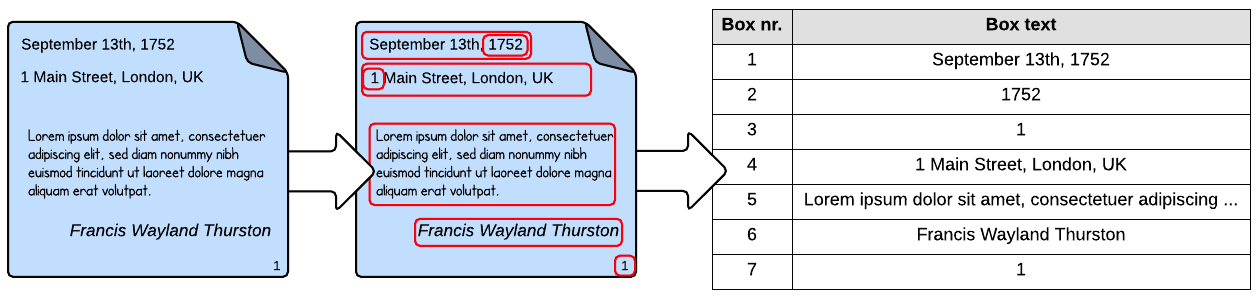
\includegraphics[width=0.9\textwidth]{FeatureExtraction1.png}
			\end{center}
			\caption{Document segmentation from Kaggle website 
			\label{fig:FeatureExtraction1}}
		\end{figure}

	\end{frame}

	%#########################################
	%##  input vector
	\begin{frame}{Competition description}

	\begin{figure}
	    \resizebox{\columnwidth}{!}{
			\begin{tabular}{ccccccccccc}
				id & x1 & x2 & x3 & x4 & x5 & x6 & x7\\ 
				1 & NO & NO & dqOiM6y(...)8= & GNjrXXA(...)= & 0.57656116338 & 0.073139435414 \\
				\hline
				x8 & x9 & x10 & x11 & x12 & x13 & x14 & x15 \\
				0.11569717707 & 0.47247428917 & YES & NO & NO & NO & NO & 42 \\
				\hline
				x16 & x17 & x18 & x19 & x20 & x21 & x22 & x23 \\
				0.3960650128 & 3 & 6 & 0.99101796407 & 0 & 0.82 & 3306 & 4676 \\
				\hline
				x24 & x25 & x26 & x27 & x28 & x29 & x30 & x31 \\
				YES & NO & YES & 0 & 0.40504704875 & 0.46460980036 & NO & NO \\
				\hline
				x32 & x33 & x34 & x35 & x36 & x37 & x38 & x39 \\
				NO & NO & mimucPm(...)= & s7mTY62(...)= & 0.57656116338 & 0.073139435414 & 0.48139435414 & 0.11569717707 \\
				\hline
				x40 & x41 & x42 & x43 & x44 & x45 & x46 & x47 \\
				0.45856019358 & YES & NO & YES & NO & NO & 9 & 0.36826347305 \\
				\hline
				x48 & x49 & x50 & x51 & x52 & x53 & x54 & x55 \\
				2 & 10 & 0.99272882805 & 0 & 0.94 & 3306 & 4676 & YES \\
			\end{tabular}
		}
		\caption{Extract of 55 (out of 145) features of sample 1 given by \textit{Tradeshift} }
		\label{fig:inputVector}
	\end{figure}

	\end{frame}


	%#########################################
	%##  output vector
	\begin{frame}{Competition description}

		\begin{figure}
			\centering
			\begin{tabular}{ccccccccccccccccccccccccccccc}
				id & y1 & y2 & y3 & y4 & y5 & y6 & y7 & y8 & y9 & y10 & y11 \\ 
				1 & 0 & 0 & 0 & 0 & 0 & 0 & 0 & 0 & 0 & 0 & 0 \\
				\hline
				y12 & y13 & y14 & y15 & y16 & y17 & y18 & y19 & y20 & y21 & y22 & y23 \\
				0 & 0 & 0 & 0 & 0 & 0 & 0 & 0 & 0 & 0 & 0 & 0 \\
				\hline
				&y24 & y25 & y26 & y27 & y28 & y29 & y30 & y31 & y32 & y33 \\
				&0 & 0 & 0 & 0 & 0 & 0 & 0 & 0 & 0 & 1
			\end{tabular}
			\caption{Labels of sample 1 given by \textit{Tradeshift}}
			\label{fig:sample1_labels}
		\end{figure}

	\end{frame}


	%#########################################
	%##  remark
	\begin{frame}{Remark on the data}

		\visible<1->{The five block hypothesis.}

		\visible<2->{

			\begin{figure}
			    \resizebox{\columnwidth}{!}{
					\begin{tabular}{ccccccccccccccccccccccccccccc}
						x1 & x2 & x3 & x4 & x5 & x6 & x7 & x8 & x9 & x10 & x11 & x12 & x13 & x14 & x15 \\ x16 & x17 & x18 & x19 & x20 & x21 & x22 & x23 & x24 & x25 & x26 & x27 & x28 & x29 \\
						NO & NO & dqOiM6(...)= & GNjrXX(...)= & 0.57656 & 0.07313 & 0.48139 & 0.11569 & 0.47247 & YES & NO & NO & NO & NO & 42 \\ 0.39606 & 3 & 6 & 0.99101 & 0 & 0.82 & 3306 & 4676 & YES & NO & YES & 0 & 0.40504 & 0.464609 \\
						\hline
						x32 & x33 & x34 & x35 & x36 & x37 & x38 & x39 & x40 & x41 & x42 & x43 & x44 & x45 & x46 \\ x47 & x48 & x49 & x50 & x51 & x52 & x53 & x54 & x55 & x56 & x57 & x58 & x59 & x60 \\
						NO & NO & mimucP(...)= & s7mTY6(...)= & 0.57656 & 0.07313 & 0.48139 & 0.11569 & 0.45856 & YES & NO & YES & NO & NO & 9 \\ 0.36826 & 2 & 10 & 0.99272 & 0 & 0.94 & 3306 & 4676 & YES & NO & YES & 1 & 0.3755 & 0.451300 \\
						\hline
						x62 & x63 & x64 & x65 & x66 & x67 & x68 & x69 & x70 & x71 & x72 & x73 & x74 & x75 & x76 \\ x77 & x78 & x79 & x80 & x81 & x82 & x83 & x84 & x85 & x86 & x87 & x88 & x89 & x90 \\
						NO & NO & Op+X3a(...)= & GeerC2(...)= & 0.57656 & 0.07313 & 0.48139 & 0.11569 & 0.48759 & YES & NO & NO & NO & NO & 42 \\ 0.36313 & 6 & 10 & 0.98759 & 0 & 0.71 & 3306 & 4676 & YES & NO & YES & 0 & 0.3755 & 0.479733 \\
						\hline
						x92 & x93 & x94 & x95 & x96 & x97 & x98 & x99 & x100 & x101 & x102 & x103 & x104 & x105 & x106 \\ x107 & x108 & x109 & x110 & x111 & x112 & x113 & x114 & x115 & x116 & x117 & x118 & x119 & x120 \\
						NO & NO & +dia7t(...)= & f4Uu1R(...)= & 0.57656 & 0.07313 & 0.48139 & 0.11569 & 0.47307 & YES & NO & NO & NO & NO & 37 \\ 0.33361 & 4 & 6 & 0.98716 & 0 & 0.89 & 3306 & 4676 & YES & NO & YES & 1 & 0.34644 & 0.464609 \\
						\hline
						x30 & x31 & x61 & x91 & x121 & x122 & x123 & x124 & x125 & x126 & x127 & x128 & x129 & x130 & x131 \\ x132 & x133 & x134 & x135 & x136 & x137 & x138 & x139 & x140 & x141 & x142 & x143 & x144 & x145 \\
						NO & NO & +2TNtX(...)= & bxU52t(...)= & 0.57656 & 0.07313 & 0.48139 & 0.11569 & 0.47307 & YES & NO & NO & NO & NO & 42 \\ 0.36313 & 5 & 6 & 0.98759 & 0 & 0.81 & 3306 & 4676 & YES & NO & YES & 2 & 0.3755 & 0.464609 \\
					\end{tabular}
				}
				\caption{First sample in a five bloc format}
				\label{fig:sample1_block}
			\end{figure}

		}

	\end{frame}





	%####################################################################################################### 
	%####################################################################################################### PROPOSED MODEL
	%####################################################################################################### 



	%#########################################
	%##  Logistic regression model
	\section{Classifier}
	\subsection{Logistic regression model}
	\begin{frame}{Logistic regression model}

		\visible<1->{

			\begin{figure}
				\centering
				\def\layersep{3em}

				\begin{tikzpicture}[shorten >=1pt,->,draw=black!50, node distance=\layersep]
					\tikzstyle{every pin edge}=[<-, thick,shorten >=1pt]
					\tikzstyle{neuron}=[circle,draw=black, very thick,,minimum size=1.5em,inner sep=0em]
					\tikzstyle{annot} = [text width=9em, text centered]
					\tikzstyle{annot2} = [text width=6em, text centered]

					% --------------
					%   Draw nodes
					% --------------
					\node[neuron] (O) at (3.5,\layersep*3) {}; % Draw output node

					\foreach \name / \y in {1,...,6} % Draw the inputs nodes
						\node[neuron] (H2-\name) at (\y+0.0,\layersep*2) {};

					% -----------------
					%   Connect nodes
					% -----------------
					\foreach \source in {1,...,6} % connect inputs & out
							\path (H2-\source) edge (O);

				\end{tikzpicture}

				\caption{Example of logistic regression model}
				\label{fig:DNN}
			\end{figure}
		}

		\vskip 1cm

		\visible<2->{

			\begin{columns}[c]
				\column{.3\textwidth}
				Aggregate weights
				$$ \sum_{j=1}^m \beta_j x_{ij}  = \beta^T x_i $$

				\column{.3\textwidth}
				Sigmoid function
				$$ \sigma(\beta,x) = \frac{ 1 }{1 + e^{-\beta^T x_i} } $$

			\end{columns}

		}


	\end{frame}


	% %#########################################
	% %##  Maximum-likelihood
	% \begin{frame}{Maximum-likelihood}


	% 	\begin{block}{Likelihood function}
	% 		The likelihood expresses the probability of the observed data as a function of the unknown parameters.\footnote{"Applied logistic regression" by Hosmer and Lemeshow p.8}
	% 		$$ l(\beta_i) = P(Y=1|x_i)^{y_i} [ 1 - P(Y=0|x_i) ]^{1-y_i} $$
	% 	\end{block}


	% \end{frame}


	%#########################################
	%##  Maximum-likelihood
	\begin{frame}{Evaluation Criterion}


		\begin{block}{Negative Log-likelihood function}
			The Negative Log-likelihood function expresses the negative of log probability of the observed data as a function of the unknown parameters.
			$$ f(\beta) = -\ln(l(\beta)) = -\sum_{i=1}^n [ y_i \ln(\hat{y_i})+ (1-y_i)\ln(1-\hat{y_i})] $$
			Where $\hat{y} $ is $P(Y=1|x_i)$ when ${y_i}=1$ and $P(Y=0|x_i)$ when ${y_i}=0$
		\end{block}


	\end{frame}


	%#########################################
	%##  Gradient descent
	\subsection{Descent Algorithm}
	\begin{frame}{Gradient Descent}

		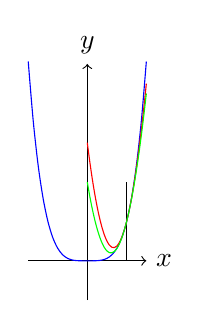
\begin{tikzpicture}[scale=0.50]
			\draw[->] (-1.5,0) -- ((1.5,0) node[right] {$x$};
			\draw[->] (0,-1) -- (0,5) node[above] {$y$};
			\draw[] (1,0) -- (1,2) node[above] {};

			\draw[scale=1,domain=-1.5:1.5,smooth,variable=\x,blue] plot ({\x},{\x*\x*\x*\x});
			\visible<2->{\draw[scale=1,domain=0:1.5,smooth,variable=\x,red] plot ({\x},{6*\x*\x-8*\x+3}); }
			\visible<3->{\draw[scale=1,domain=0:1.5,smooth,variable=\x,green] plot ({\x},{5*\x*\x-6*\x+2}); }

		\end{tikzpicture}

		\visible<2->{\textbf{example}\\
		f(x) = $x^4$. We consider the point $x_t=1$\\ 
		Quadratic approximation : $ f_q(x) = f(x_t) + f'(x_t)(x-x_t) + \frac{f''(x_t)}{2} (x-x_t)^2 $\\}
		\visible<3->{GD approximation : $ f_o(x) = f(x_t) + f'(x_t)(x-x_t) + \frac{1}{2\alpha} \norm{x-x_t}_2^2 $\\ }

		\visible<4->{ $$ x_{t+1} = x_t - \alpha \nabla f(x_t)$$ }		


	\end{frame}


	% %#########################################
	% %##  Gradient descent
	% \begin{frame}{Gradient Descent}

	% 	\visible<1->{Gradient Descent : $$ x_{t+1} = \argmin_x f(x_t)+ \nabla f(x_t)^T \cdot (x-x_t) + \frac{1}{2\alpha}\norm{x-x_t}_2^2 $$}

	% 	\visible<2->{Mirror Descent : $$ x_{t+1} = \argmin_x f(x_t)+\nabla f(x_t)^T(x-x_t) + \Delta B_{1:t}(x,x_t)  $$}

	% 	\visible<3->{COMID : $$ x_{t+1} = \argmin_x f(x_t)+\nabla f(x_t)^T(x-x_t) + \Delta B_{1:t}(x,x_t) + \Psi(x) $$}

	% 	\visible<4->{FTPRL is similar to COMID but has a adaptive regularization.}

	% \end{frame}


	%#########################################
	%##  feature selection
	\subsection{Feature selection}
	\begin{frame}{Feature selection}

		\begin{figure}
			\centering
			\def\layersep{3em}

			\begin{tikzpicture}[shorten >=1pt,->,draw=black!50, node distance=\layersep]
				\tikzstyle{every pin edge}=[<-, thick,shorten >=1pt]
				\tikzstyle{neuron}=[circle,draw=black, very thick,,minimum size=1.5em,inner sep=0em]
				\tikzstyle{annot} = [text width=9em, text centered]
				\tikzstyle{annot2} = [text width=6em, text centered]

				% --------------
				%   Draw nodes
				% --------------
				\node[neuron] (O) at (2,\layersep*3) {}; % Draw output node

				\node[neuron] (H2-1) at (1+0.0,\layersep*2) {A};
				\node[neuron] (H2-2) at (2+0.0,\layersep*2) {B};
				\node[neuron] (H2-3) at (3+0.0,\layersep*2) {C};


				% -----------------
				%   Connect nodes
				% -----------------
				\foreach \source in {1,...,3} % connect inputs & out
						\path (H2-\source) edge (O);

			\end{tikzpicture}

			\caption{Example of logistic regression model}
			\label{fig:DNN}
		\end{figure}


		\begin{columns}
			\column{.3\textwidth}
			\begin{itemize}
				\item<2-> Test \{A\}
				\item<2-> Test \{B\}
				\item<2-> Test \{C\}
			\end{itemize}

			\column{.3\textwidth}
			\begin{itemize}
				\item<3-> Test \{BA\}
				\item<3-> Test \{BC\}
			\end{itemize}

			\column{.3\textwidth}
			\begin{itemize}
				\item<4-> Test \{BCA\}
			\end{itemize}
		\end{columns}


	\end{frame}




	%####################################################################################################### 
	%####################################################################################################### PROPOSED FEATURES
	%####################################################################################################### 


	%#########################################
	%##  Feature-engineering
	\section{Feature-engineering}
	\begin{frame}{Feature-engineering}

		\begin{block}{Data normalization}
			Feature standardization : perform a mean-subtraction then set the variance to a unit variance.
		\end{block}

		\vskip 1cm

		\visible<2->{
			\begin{table}
				\centering
				\begin{tabular}{c|c|c}
					Algorithm 			 & $x=18$ & $x=17$ \\
					\hline
					FTPRL[x]\_no\_norm		& 0.195626763424 & 0.204790168023 \\
					FTPRL[x]\_classic\_norm	& 0.199563944287 & 0.242193956451 \\
					FTPRL[x]\_5\_bloc\_norm	& 0.199563944287 & 0.242193956451 \\
				\end{tabular}
				\caption{Model results given the normalization. [x] stands for the feature it has been training on.}
				\label{tab:normalization}
			\end{table}
		}

	\end{frame}




	%#########################################
	%##  FTPRL_feat_1hot
	\begin{frame}{Feature-engineering}

			\begin{block}{Data normalization}
			Feature standardization : perform a mean-subtraction then set the variance to a unit variance.
		\end{block}

		\vskip 1cm

		\begin{table}
			\resizebox{\columnwidth}{!}{
				\begin{tabular}{c|c|c|c|c|c|c|c|c|c}
					step i = & 1  & 2 & 3 & 4 & 5 & 6 & 7 & 8 & 9\\
					\hline
					New feature 			 & [18] & [2] & [21] & [11] & [7] & [25] & [19] & [16] & [9] \\
					FTPRL\_feat	&  .1995 & .1819 & .161 & .1509 & .1414 & .1342 & .1293 & .1248 & .1224   \\
				\end{tabular}
			}	
			\caption{Result of feeding FSSFTPRL with all the initial normalized features. At step "i" the model choses a new feature to learn with (FSS) }
			\label{tab:FTPRL_feat}
		\end{table}
		
	\end{frame}


	%#########################################
	%##  FTPRL_feat_1hot
	\begin{frame}{Feature-engineering}

		\begin{block}{One-hot feature encoding}
			Is a representation of a feature. We create a vector full of zeros with as many dimentions than the original feature has values. Then add a zero on the new vector at the sample value index.
			$$ [5] => [0,0,0,0,0,1,0] $$
		\end{block}

		\vskip 1cm

		\visible<2->{
			\begin{table}
				\centering
				\begin{tabular}{c|c|c|c}
					step i = & 1 & 2 & 3 \\
					\hline
					New feature 		& \{17\} & \{4\} & \{3\}    \\
					FTPRL\_feat\_1hot	&  0.0824 & 0.0722 & 0.0662 \\
				\end{tabular}
				\caption{Result of feeding FSSFTPRL with all the one-hotted features . At step "i" the model choses a new feature to learn with (FSS). \{x\} stands for one-hotted feature [x]  }
				\label{tab:FTPRL_feat_1hot}
			\end{table}
		}
	\end{frame}


	%#########################################
	%##  FTPRL_feat_HEFV
	\begin{frame}{Feature-engineering}

		\begin{block}{Hash Equality Feature Vector}
			Create a one-hot vector symbolizing the hash pairs equalities in a sample.
		\end{block}

		\vskip 1cm

		\visible<2->{
			\begin{table}
				\centering
				\begin{tabular}{c|c|c|c|c|c}
					step i = & 1 & 2 & 3 & 4 & 5 \\
					\hline
					New feature 		& [18] & HEFV & [25] & [1] & [11] \\
					FTPRL\_feat\_HEFV	&  .1995 & .0965 & .0883 & .0851 & .0837 \\
				\end{tabular}
				\caption{Result of feeding FSSFTPRL with all the initial normalized features and HEFV. At step "i" the model choses a new feature to learn with (FSS).  }
				\label{tab:FTPRL_feat_HEFV}
			\end{table}
		}
	\end{frame}


	%#########################################
	%##  FTPRL_feat_FEFV
	\begin{frame}{Feature-engineering}

		\begin{block}{Features Equality Feature Vector}
			Create a one-hot vector symbolizing the Features pairs equalities in a sample.
		\end{block}

		\vskip 1cm

		\visible<2->{
			\begin{table}
				\centering
				\begin{tabular}{c|c|c|c}
					step i = & 1 & 2 & 3  \\
					\hline
					New feature 	&	FEFV & [18] & [17] \\
					FTPRL\_feat\_FEFV	&  .1053 & .1003 & .0846 \\
				\end{tabular}
				\caption{Result of feeding FSSFTPRL with all the initial normalized features and FEFV. At step "i" the model choses a new feature to learn with (FSS).  }
				\label{tab:FTPRL_feat_FEFV}
				\end{table}
			}
	\end{frame}


	%#########################################
	%##  FTPRL_all
	\begin{frame}{Feature-engineering}

		\begin{block}{Try all the new features}
			Test the model with all the features presented above.
		\end{block}

		\vskip 1cm

		\visible<2->{
			\begin{table}
				\centering
				\begin{tabular}{c|c|c|c|c}
					step i = & 1 & 2 & 3 & 4 \\
					\hline
					New feature 	& \{17\} & \{4\} & \{3\} & HEFV \\
					FTPRL\_all	&  0.0824 & 0.0722 & 0.0662 & .0576\\
				\end{tabular}
				\caption{Result of feeding FSSFTPRL with all features seen so far. }
				\label{tab:FTPRL_all}
			\end{table}
		}
	\end{frame}


	%#########################################
	%## Conclusion
	\section{Conclusion}
	\begin{frame}{Conclusion}

		\visible<1->{
			\begin{itemize}
				\item Implement a linear regression model corresponding to the problematic.
				\item Hand-engineer features.
				\item Perform better with new features.
			\end{itemize}
		}

		\vskip 1cm

		\visible<2->{
			\begin{block}{Future work}
				Try this method on an other dataset.
			\end{block}
		}

	\end{frame}



\appendix


	%#########################################
	%##  Gradient descent
	\begin{frame}
		\titlepage
	\end{frame}

	%#########################################
	%##  Gradient descent
	\begin{frame}{Gradient Descent}

		\visible<1->{Gradient Descent : $$ x_{t+1} = \argmin_x f(x_t)+ \nabla f(x_t)^T \cdot (x-x_t) + \frac{1}{2\alpha}\norm{x-x_t}_2^2 $$}

		\visible<2->{Mirror Descent : $$ x_{t+1} = \argmin_x f(x_t)+\nabla f(x_t)^T(x-x_t) + \Delta B_{1:t}(x,x_t)  $$}

		\visible<3->{COMID : $$ x_{t+1} = \argmin_x f(x_t)+\nabla f(x_t)^T(x-x_t) + \Delta B_{1:t}(x,x_t) + \Psi(x) $$}

		\visible<4->{FTPRL is similar to COMID but has a adaptive regularization.}

	\end{frame}






\end{document}




